\documentclass[12pt,a4paper]{article}
\usepackage{cite}
\usepackage{amsmath,amssymb,amsfonts,amsthm}
\usepackage{algorithmic}
\usepackage{graphicx}
\usepackage{textcomp}
\usepackage{xcolor}
\usepackage{txfonts}
\usepackage{algorithm}
\usepackage{algpseudocode}
\usepackage{listings}
\usepackage{enumitem}
\usepackage{mathtools}
\usepackage{gensymb}
\usepackage{comment}
\usepackage[breaklinks=true]{hyperref}
\usepackage{tkz-euclide} 
\usepackage{listings}
\usepackage{multicol}
\usepackage{xparse}
\usepackage{gvv}
%\def\inputGnumericTable{}                                 
\usepackage[latin1]{inputenc}                                
\usepackage{color}                                            
\usepackage{array}                                            
\usepackage{longtable}                                       
\usepackage{calc}                                             
\usepackage{multirow}                                         
\usepackage{hhline}                                           
\usepackage{ifthen}                                               
\usepackage{lscape}
\usepackage{tabularx}
\usepackage{array}
\usepackage{float}
\usepackage{ar}
\usepackage[version=4]{mhchem}
\setlength{\parindent}{0pt}
\setlength{\parskip}{1em}

\title{\textbf{Software Assignment Report}\\[10pt]
\textbf{IMAGE COMPRESSION USING TRUNCATED SVD}}
\author{Avaneesh - EE25BTECH11030}
\date{November 7, 2025}

\begin{document}

\maketitle
\newpage

\section*{Introduction}
  Singular Value Decomposition(SVD) is a decomposition of a rectangular matrix into three easily interpretable matrices.\\SVD is one of the most powerful and versatile tools in applied mathematics, machine learning, and signal processing because it gives deep insight into a matrix’s structure, stability, and dimensionality.


\section*{Summary of Strang's video}
\begin{itemize}
\item SVD is the best decomposition as it can be done for any matrix.
\item A rectangular matrix $A$ is decomposed into three matrices $U,V,\Sigma$ where $U , V$ are orthogonal matrices and $\Sigma$ is a diagonal matrix with its entries comprising singular values in descending order.$$A=U\Sigma V^{\top}$$ $U$ is left singular matrix and $V$ is right singular matrix.
\item In case of symmetric positive definite matrix $S$, it can be decomposed as $$S=Q\Lambda Q^{\top}$$
where $Q$ is orthogonal matrix and $\Lambda$ is diagonal matrix containing Eigen values of the symmetric matrix.
\item Let $A\in \mathbb{R}^{n\times n}$ where $n\geq m$ and $U\in \mathbb{R}^{n\times r} , V\in \mathbb{R}^{n\times r}, \Sigma \in \mathbb{R}^{r\times r}$ \begin{align*}
    A^{\top}A&=\left(U\Sigma V^{\top}\right)\left(U\Sigma V^{\top}\right)=V\Sigma ^{\top}U^{\top} U\Sigma V^{\top}\\
    &=V\Sigma^{\top}\Sigma V^{\top}=V\Sigma ^{2} V^{\top}
\end{align*}
$A^{\top}A$ is sym and positive definite matrix, so $V$ is matrix containing eigen vectors of $A^{\top}A$ and $\Sigma ^2$ the diagonal values are eigen values of $A^{\top}A$\\
Similarly, $U$ contains eigen vectors of matrix $AA^{\top}$.
\item We get $$A\myvec{V_1&&V_2&&...&&V_r}=\myvec{u_1&&u_2&&...&&u_r}\myvec{\sigma_1&&0&&...\\0&&\sigma_2&&...\\..&&..&&..}$$
where $\sigma_1\geq \sigma_2 \geq ...\geq 0$

\item product of eigen values = $det(A)$\\product of singular values = $det(A)$
\item The value of $u_1 \Sigma_1v_1^{\top}$ is the most dominant and important data in the matrix.

\end{itemize}


\section*{Math}

\begin{itemize}
    \item Given a matrix $A$ we need to calculate the matrix $A_k$ which is the frobenius norm $\norm{A-A_k}$ is minimum.
    \item For this I am using "Power Iteration with Deflation" method to solve for SVD to calculate the first k singular values $\brak{\sigma_1,\sigma_2,.. , \sigma_k}$.
    \item We need to find $$A_k=U_k\Sigma_k V_k^{\top}$$
    \item In this method I am first calculating the eigen vectors of $A^{\top}A$ which are the right singular vectors of $A$.\\
    Let $B=A^{\top}A$, and the eigen values of $B$ are $e_1,e_2,..$.
    \item Now take a random vector $\vec{v_1}= b_1e_1+b_2e_2+.. $ where $b_1,b_2,..$ are some constants.\\
    Consider a new vector $$v_{new}=Bv_1$$
    $$v_{new}=b_1Be_1+b_2Be_2+..$$
    as $e$ are the eigen vectors of $B$, $Be_1=\lambda_1e_1$ where $\lambda_1$ is the eigen value of $e_1$.
    $$v_{new}=b_1\lambda_1e_1+b_2\lambda_2e_2+..$$
    After finding $v_{new}$ I am normalizing it.
    \item This step I am implementing repeatedly (about 20 - 30 times is sufficient) which makes the $v_{new}$ with the eigen vector with the most dominant eigen value.In this way i was able to find the most important right singular vector.\\
    Now $v_{new}=v_1$\\
    For $\sigma_1=\sqrt{\lambda_1}$ where $\lambda_1=\norm{v_{1}}$.
    \item For the remaining k-1 right singular vectors I will deflate the matrix $B$ with the $v_{1}$ that I found in the before step.(i.e changing the matrix such that its singular value for $v_{1}$ will be 0.)\\
    This matrix $B$ is changed to $B-\lambda_1v_1v_1^{\top}$
    \item We can prove this by multiplying with vector $\vec{v_1}$ on both sides.
    $$Bv_1-\lambda_1v_1v_1^{\top}v_1=0$$
    Hence we removed the component of $v_1$ from B.

    \item This same process is continued until the k right singular vectors and corresponding singular values are found and can form matrix $V_k$ containg columns as the right singular vectors and $\Sigma_k$ containing all diagonal entries as the singular values in descending order.
    \item We can find the vectors $u_1,u_2,.. $ by $$u_1=\frac{Av_1}{\sigma_1}, ..$$
    and hence form the matrix $U_k$ containing the columns as $u_1,u_2,..$.
    \item The output matrix=$U_k\Sigma_k v_k^{\top}$
\end{itemize}

\section*{Pseudo Code}

\begin{algorithm}[H]
\caption{Power Iteration: \textsc{maxlambda(B, n)}}
\label{algorithm:max_lambda}
\Require Symmetric matrix $B \in \mathbb{R}^{n \times n}$
\Ensure Dominant eigenvector $v$ and corresponding eigenvalue $\lambda_{max}$

\State $v \gets \text{random vector of size } n$
\State $v \gets v / \norm{v}$ \Comment{Normalize the initial vector}

\For{$i = 1 \to 25$} \Comment{number of iteration}
    \State $v_{new} \gets Bv$
    \State $v \gets v_{new} / \norm{v_{new}}$ \Comment{Normalize the new vector}
\EndFor

\State $\lambda_{max} \gets v^\top (Bv)$ \Comment{This is Rayleigh Quotient}
\State \Return $v$, $\lambda_{max}$
\end{algorithm}

\begin{algorithm}[H]
\caption{Truncated SVD with Deflation: \textsc{SVDtruncated(A, k)}}
\label{algorithm:svd}
\Require Matrix $A \in \mathbb{R}^{n \times m}$, rank $k$
\Ensure Matrices $U_k \in \mathbb{R}^{n \times k}$, $S_k \in \mathbb{R}^{k}$, $V_k \in \mathbb{R}^{m \times k}$

\State Initialize $U_k$, $S_k$, $V_k$
\State $B \gets A^\top A$ 

\For{$i = 1 \to k$}
    \State $(v, \lambda) \gets \textsc{maxlambda}(B, m)$ \Comment{Find dominant component}
    
    \State $\sigma \gets \sqrt{\max(0, \lambda)}$ \Comment{so that there is no negative value under root}
    \State $S_k[i] \gets \sigma$ \Comment{Store singular value (as a vector)}
    \State $V_k[i] \gets v$ \Comment{Set i-th column of $V_k$ as v}
    
    \State $u \gets Av$
    \State $\sigma \gets \max(\sigma, 10^{-12})$ \Comment{Avoid division by zero}
    \State $u \gets u / \sigma$
    \State $U_k[i] \gets u$ \Comment{Set i-th column of $U_k$ as u}
    
    \State $B \gets B - \lambda v v^\top$ \Comment{Deflation of the matrix}
\EndFor
\State \Return $U_k$, $S_k$, $V_k$
\end{algorithm}

\begin{algorithm}[H]
\caption{Image Reconstruction: \textsc{Reconstructimage}(U_k, S_k, V_k)}
\label{algorithm:reconstruct}
\Require $U_k \in \mathbb{R}^{n \times k}$, $S_k \in \mathbb{R}^{k}$, $V_k \in \mathbb{R}^{m \times k}$
\Ensure Reconstructed matrix $A_k \in \mathbb{R}^{n \times m}$

\State $Sk\_diag \gets \text{diag}(S_k)$ \Comment{Create $k \times k$ diagonal matrix from $S_k$ whose diagonal entries are entries of $S_k$}
\State $A_{k} \gets U_k Sk\_diag  V_k^\top$ \Comment{Reconstructing the output matrix}
\State \Return $A_{k}$
\end{algorithm}

\newpage
\section*{Different Algorithms for computing SVD}
There are four common methods for computing SVD:

\section{Golub-Kahan-Reinsch (GKR)}

\subsection*{Definition}
It is the "gold standard" algorithm.It is used in making multiple libraries like LAPACK (which is used by NumPy, MATLAB, etc.) which uses SVD. It is a two-phase algorithm:
\begin{enumerate}
    \item \textbf{Bidiagonalization:} Here, the matrix $A$ is reduced to an upper bidiagonal matrix $B$ using a series of Householder reflections.
    \item \textbf{QR Iteration:} It is a variant of the QR algorithm which is iteratively applied to $B$ to find its singular values, which are the same as $A$'s singular values.
\end{enumerate}
This is the breif explanation on GKR.

\subsection*{Advantages}
\begin{itemize}
    \item \textbf{Numerically Stable}
    \item \textbf{Fast}
    \item \textbf{Guaranteed Convergence}
\end{itemize}

\subsection*{Disadvantages}
\begin{itemize}
    \item \textbf{Very Complex:} Very difficult to implement correctly from scratch.
    \item \textbf{Full SVD:} It computes the "full SVD", which is unnecessary as only the top $k$ singular values are needed for compression.
\end{itemize}

\section{Jacobi SVD}

\subsection*{Definition}
It is an iterative algorithm that applies a series of plane rotations (known as Jacobi rotations) to the matrix. The goal of this method is to apply these rotations in "sweeps" across the matrix to orthogonalize the columns (or rows). Eventually, it converges to a diagonal matrix whose diagonal entries are the singular values.
This is a breif on Jacobi 's approach.


\subsection*{Advantages}
\begin{itemize}
    \item \textbf{Simpler than GKR:} The core logic is a 2x2 rotation. This logic is much easier to understand and implement than GKR.
    \item \textbf{Accurate:} Can be very accurate, especially for small matrices.
\end{itemize}

\subsection*{Disadvantages}
\begin{itemize}
    \item \textbf{Slower:} Slower than GKR for larger matrices due to taking many sweeps for converging.
    \item \textbf{Full SVD:} Like GKR, it is a full SVD algorithm and is not useful in this case.
\end{itemize}

\section{Power Iteration with Deflation}
This is the method that I implemented which has been explained above.
\subsection*{Definition}
This is a "truncated SVD" method that finds the singular components one by one. It relies on the fact that the eigenvectors of $A^TA$ are the right singular vectors ($V$) of $A$.

\subsection*{Advantages}
\begin{itemize}
    \item \textbf{Simple to Implement:} The power iteration and deflation steps are relatively simple to implement.
    \item \textbf{Truncated SVD:} Directly computes only the top $k$ values, making it efficient if $k$ is very small.
\end{itemize}

\subsection*{Disadvantages}
\begin{itemize}
    \item \textbf{Numerically Unstable:}
        \begin{itemize}
            \item Computing $A^TA$ squares the condition numbers(which is a measure of how sensitive a function is to slight changes in inputs), which can lead to a significant loss of precision for small singular values.
            \item The deflation step accumulates numerical errors so the value of $v_k$ might have error.
        \end{itemize}
\end{itemize}

\section{Subspace Iteration (Orthogonal Iteration)}

\subsection*{Definition}
A more elegant way of "truncated SVD" method. It is essentially the power method applied to a block of $k$ vectors simultaneously.
\begin{enumerate}
    \item Start with a random $n \times k$ matrix $V$ (representing $k$ random vectors).
    \item We have to use 2 steps iteratively : power and stabilization. 
    Iterate:
        \begin{itemize}
            \item $Z = (A^TA)V$   (The "power" step: applies $B$ to all $k$ vectors).
            \item $[Q, R] = \text{qr}(Z)$     (The "stabilization" step: re-orthogonalizes the vectors via QR decomposition to prevent them all from collapsing to $v_1$).
            \item $V = Q$
        \end{itemize}
    \item The columns of the final $V$ matrix are the top $k$ singular vectors.
\end{enumerate}

\subsection*{Advantages}
\begin{itemize}
    \item \textbf{More Stable:} Vastly more numerically stable than power iteration with deflation because it avoids squaring condition number and subtraction for deflation. It uses stable QR decomposition instead.
    \item \textbf{Truncated SVD:} Efficiently finds the top $k$ values at the same time.
    
\end{itemize}

\subsection*{Disadvantages}
\begin{itemize}
    \item \textbf{More Complex:} More difficult to implement than the deflation method, as it requires  QR decomposition algorithm.
    \item \textbf{Cost of QR:} The QR decomposition step adds computational cost to each iteration.
\end{itemize}




\section*{Why I Used the Power Iteration with deflation method}
Since I want to find the matrix corresponding with only the first k singular values, this method is very easy to implement and understand.\\
The other methods are very complex to implement from scratch.\\
The Subspace Iteration method is numerically more stable but difficult to implement the QR decomposition.

\section*{Compressed Images}

\subsection{Greyscale Images}

\begin{figure}[H]
    \centering
    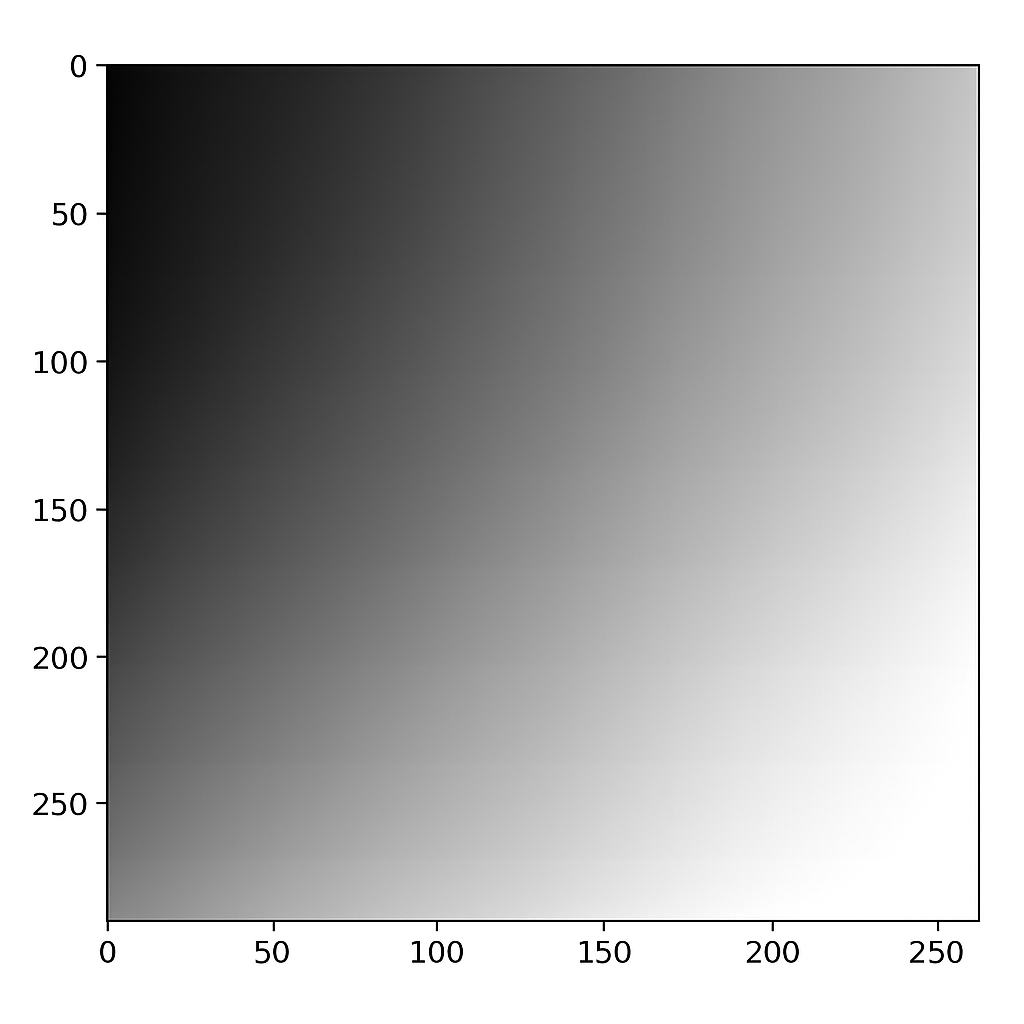
\includegraphics[width=0.5\linewidth]{figs/greyscale/greyscale.png}
    \caption{greyscale.png}
    \label{fig:1}
\end{figure}

\begin{figure}[H]
    \centering
    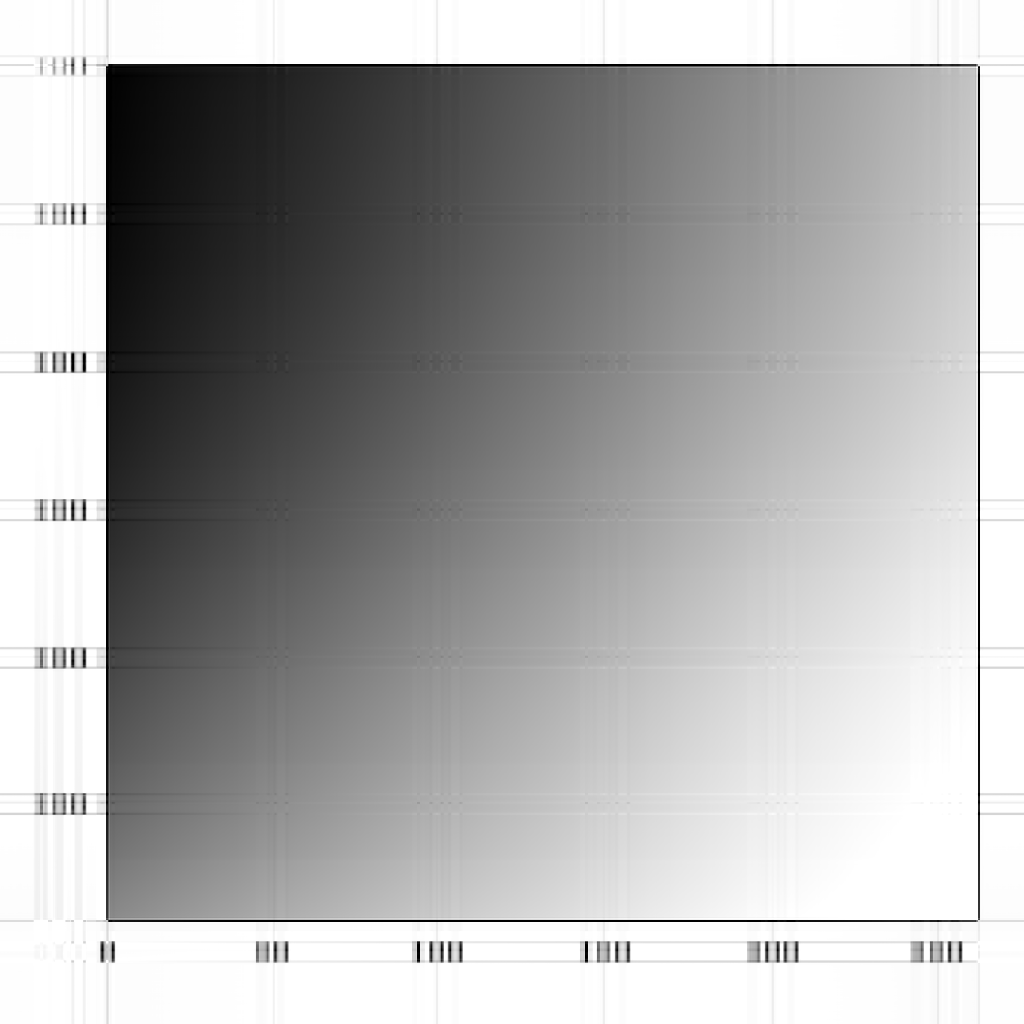
\includegraphics[width=0.5\linewidth]{figs/greyscale/greyscale5.png}
    \caption{k=5}
    \label{fig:2}
\end{figure}

\begin{figure}[H]
    \centering
    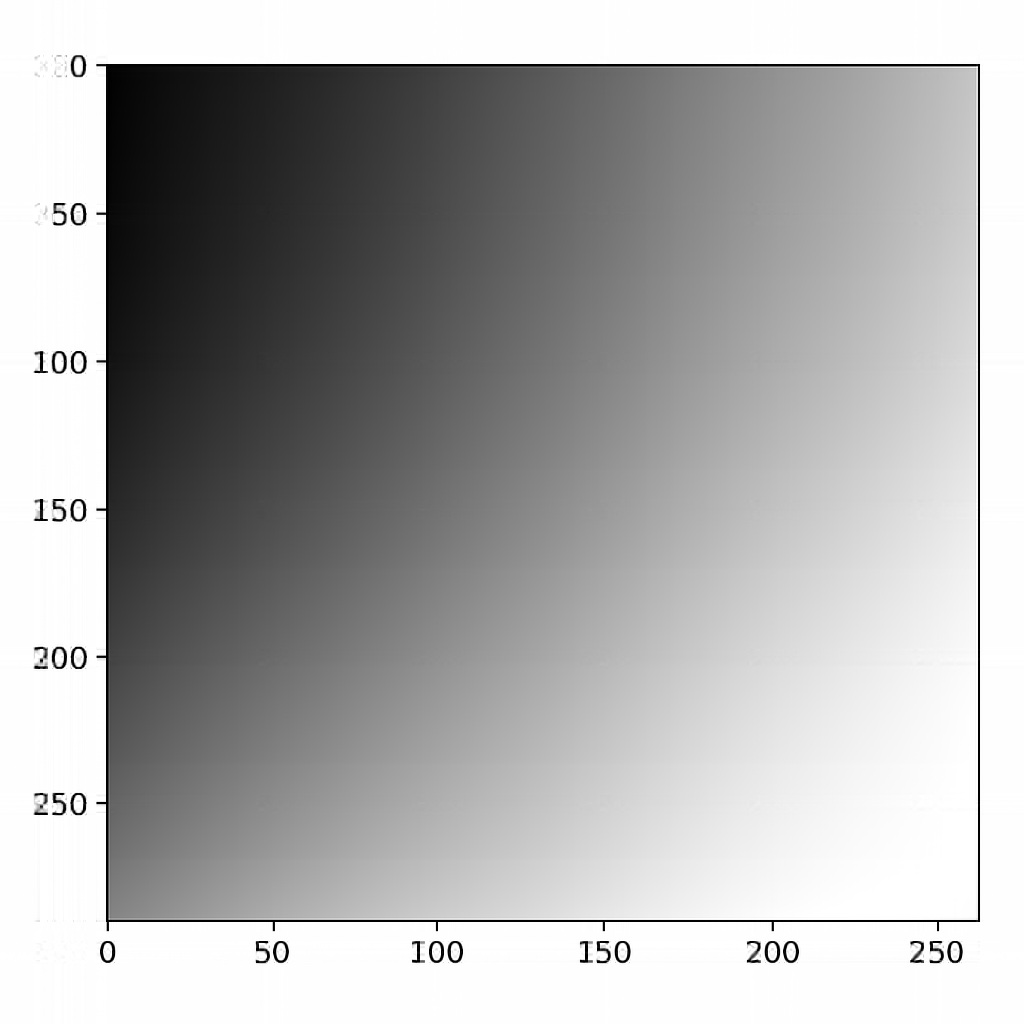
\includegraphics[width=0.5\linewidth]{figs/greyscale/greyscale20.png}
    \caption{k=20}
    \label{fig:3}
\end{figure}

\begin{figure}[H]
    \centering
    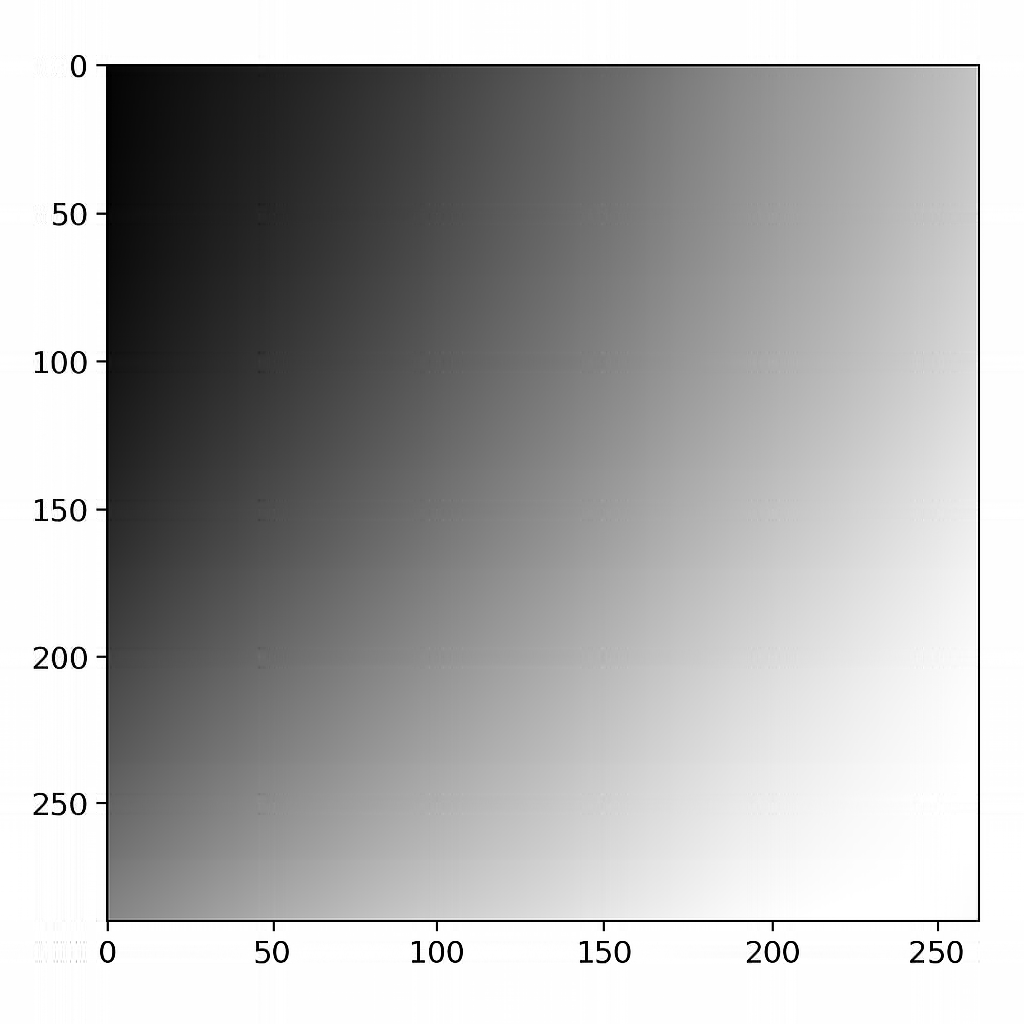
\includegraphics[width=0.5\linewidth]{figs/greyscale/greyscale50.png}
    \caption{k=50}
    \label{fig:4}
\end{figure}

\begin{figure}[H]
    \centering
    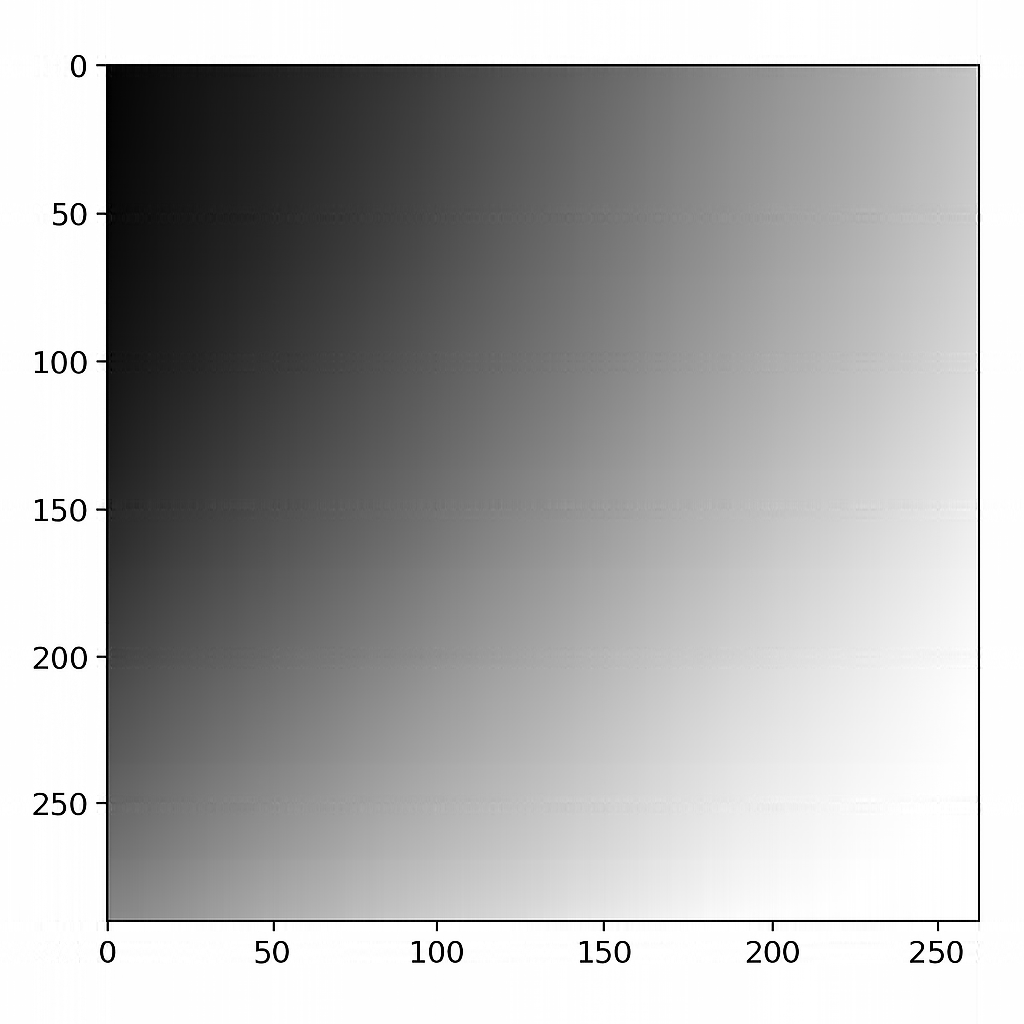
\includegraphics[width=0.5\linewidth]{figs/greyscale/greyscale100.png}
    \caption{k=100}
    \label{fig:5}
\end{figure}

\subsection{Globe Images}

\begin{figure}[H]
    \centering
    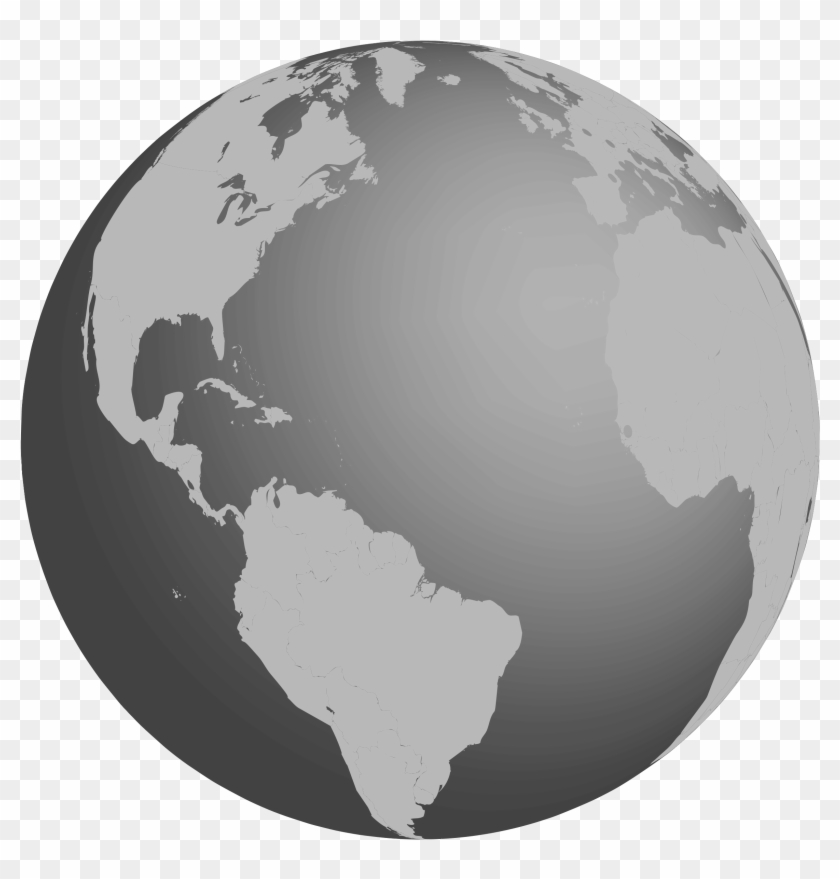
\includegraphics[width=0.5\linewidth]{figs/globe/globe.jpg}
    \caption{globe.jpg}
    \label{fig:1}
\end{figure}

\begin{figure}[H]
    \centering
    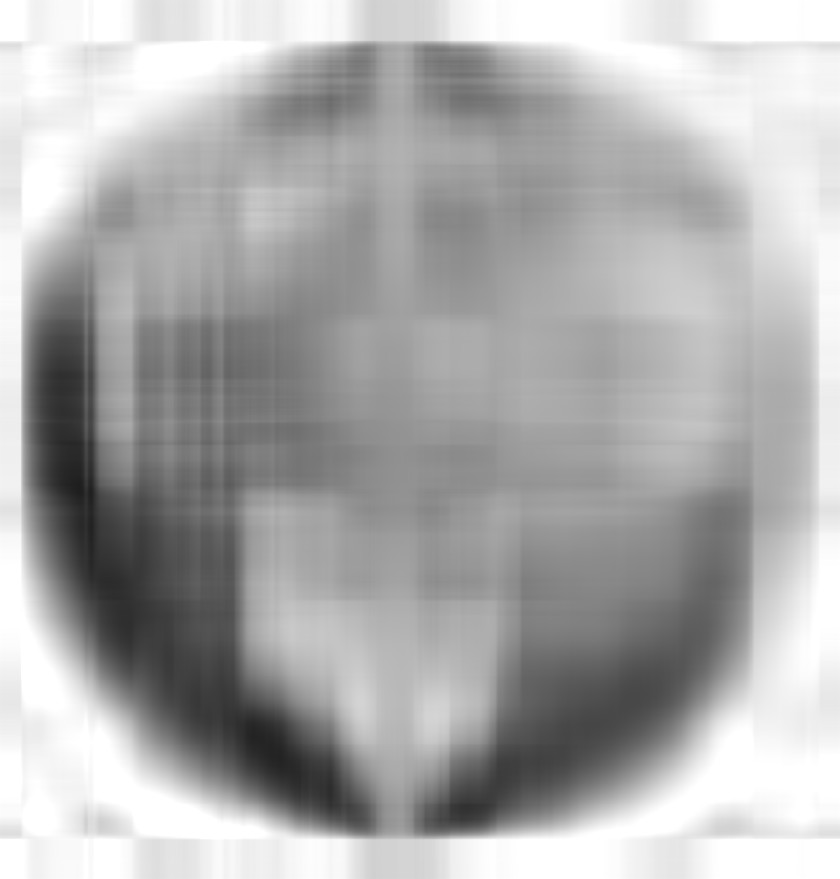
\includegraphics[width=0.5\linewidth]{figs/globe/globe5.jpg}
    \caption{k=5}
    \label{fig:2}
\end{figure}
\begin{figure}[H]
    \centering
    
\includegraphics[width=0.5\linewidth]{figs/globe/globe20.jpg}
    \caption{k=20}
    \label{fig:3}
\end{figure}

\begin{figure}[H]
    \centering
    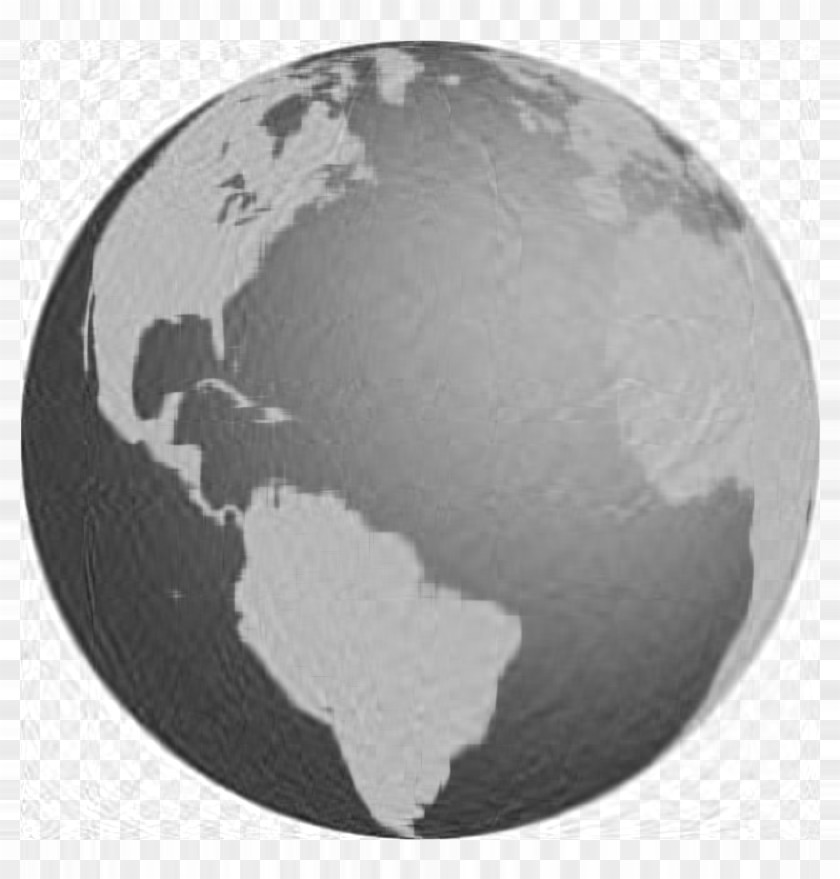
\includegraphics[width=0.5\linewidth]{figs/globe/globe50.jpg}
    \caption{k=50}
    \label{fig:4}
\end{figure}

\begin{figure}[H]
    \centering
    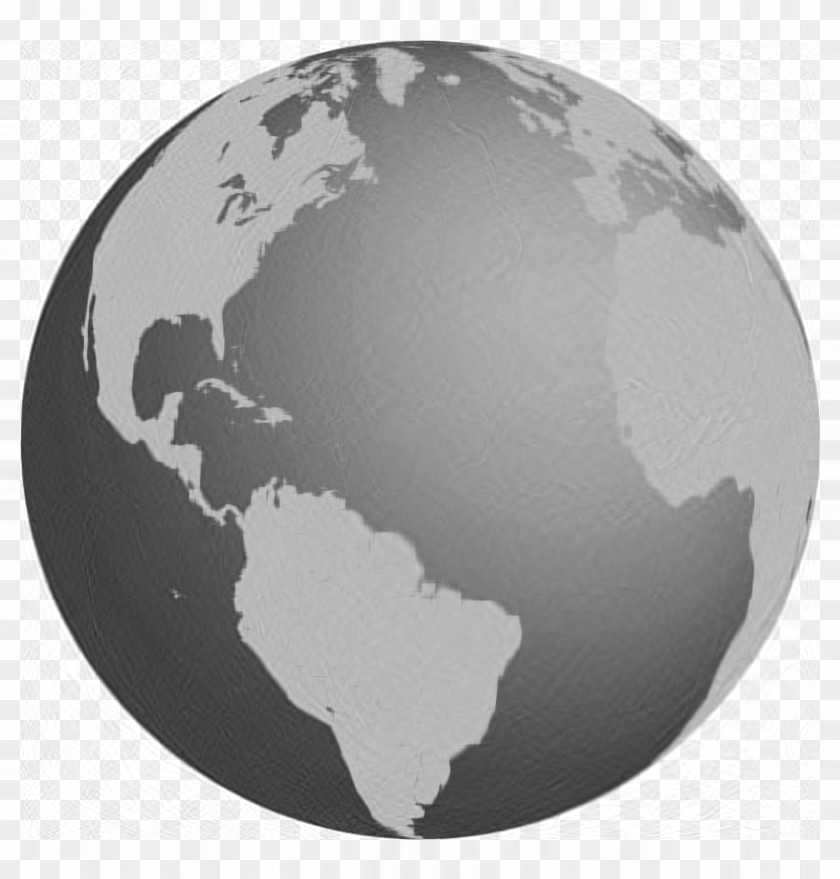
\includegraphics[width=0.5\linewidth]{figs/globe/globe100.jpg}
    \caption{k=100}
    \label{fig:5}
\end{figure}


\subsection{Einstein Images}

\begin{figure}[H]
    \centering
    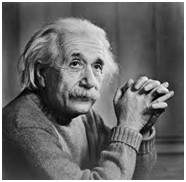
\includegraphics[width=0.5\linewidth]{figs/einstein/einstein.jpg}
    \caption{einstein.jpg}
    \label{fig:1}
\end{figure}

\begin{figure}[H]
    \centering
    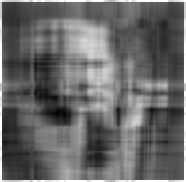
\includegraphics[width=0.5\linewidth]{figs/einstein/einstein5.jpg}
    \caption{k=5}
    \label{fig:2}
\end{figure}

\begin{figure}[H]
    \centering
    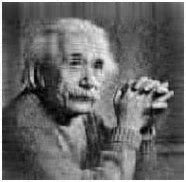
\includegraphics[width=0.5\linewidth]{figs/einstein/einstein20.jpg}
    \caption{k=20}
    \label{fig:3}
\end{figure}

\begin{figure}[H]
    \centering
    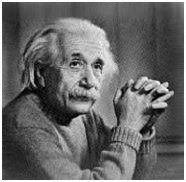
\includegraphics[width=0.5\linewidth]{figs/einstein/einstein50.jpg}
    \caption{k=50}
    \label{fig:4}
\end{figure}

\begin{figure}[H]
    \centering
    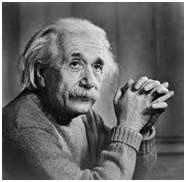
\includegraphics[width=0.5\linewidth]{figs/einstein/einstein100.jpg}
    \caption{k=100}
    \label{fig:5}
\end{figure}


\section*{Error Analysis}

The error rapidly decreases at first as $\norm{A-A_k}_F$ denotes the energy of the elements of $A$ which are not there in $A_k$. As the k values increase the amount of energy decreases in $A-A_k$. 
\begin{table}[H]
    
\centering
\begin{tabular}{|c|c|c|c|c|}
\hline
\textbf{Value of k} & \textbf{k=5} & \textbf{k=20} & \textbf{k=50} & \textbf{k=100} \\ \hline
$\norm{A-A_k}_F$ & 11146.3 & 3809.7 & 1504.1 & 981.2 \\ \hline
\end{tabular}
\caption{Frobenius Norms $\norm{A-A_k}_F$ of greyscale.png}
\label{greyscale}



\centering
\begin{tabular}{|c|c|c|c|c|}
\hline
\textbf{Value of k} & \textbf{k=5} & \textbf{k=20} & \textbf{k=50} & \textbf{k=100} \\ \hline
$\norm{A-A_k}_F$ & 20704.3 & 10636.6 & 6211.1 & 3719.2 \\ \hline
\end{tabular}
\caption{Frobenius Norms $\norm{A-A_k}_F$ of globe.jpg}
\label{globe}



\centering
\begin{tabular}{|c|c|c|c|c|}
\hline
\textbf{Value of k} & \textbf{k=5} & \textbf{k=20} & \textbf{k=50} & \textbf{k=100} \\ \hline
$\norm{A-A_k}_F$ & 4714.1 & 2127.1 & 885.0 & 199.2 \\ \hline
\end{tabular}
\caption{Frobenius Norms $\norm{A-A_k}_F$ of einstein.jpg}
\label{einstein}



\end{table}

\section*{Conclusion}
SVD is a very useful and widely used decomposition which can be used for image compression. This is my approach on using SVD for image compression of greyscale images.

\end{document}